\documentclass{chi-ext}
\copyrightinfo{ }

\title{Duo-Portal, a HTML5 cooperative game}

\numberofauthors{2}
\author{
  \alignauthor{
  	\textbf{Frederico Schardong}\\
  	\affaddr{University of Calgary}\\
  	\affaddr{Calgary, CA T2N 1N4 Canada}\\
  	\email{fschardo@ucalgary.ca}
  }\alignauthor{
  	\textbf{Cédric Guillot}\\
  	\affaddr{University of Calgary}\\
  	\affaddr{Calgary, CA T2N 1N4 Canada}\\
  	\email{cpguillo@ucalgary.ca}
  }
}

% Paper metadata (use plain text, for PDF inclusion and later re-using, if desired)
\def\plaintitle{Duo-Portal, a HTML5 cooperative game}
\def\plainauthor{Frederico Schardong}
\def\plainkeywords{Cooperative, HTML5, online game, portal}
\def\plaingeneralterms{Cooperative, HTML5, online game, portal}

\hypersetup{
  % Your metadata go here
  pdftitle={\plaintitle},
  pdfauthor={\plainauthor},  
  pdfkeywords={\plainkeywords},
  pdfsubject={\plaingeneralterms},
  % Quick access to color overriding:
  citecolor=black,
  linkcolor=blue,
  menucolor=black,
  urlcolor=blue,
}

\usepackage{graphicx}   % for EPS use the graphics package instead
\usepackage{balance}    % useful for balancing the last columns
\usepackage{bibspacing} % save vertical space in references

\begin{document}

\maketitle

\begin{abstract}
In this paper we describe the implementation of a cooperative online game in HTML5 inspired from the successful game Portal by Valve.
\end{abstract}

\category{H.5.m}{Information interfaces and presentation (e.g., HCI)}{Miscellaneous}

\terms{\plaingeneralterms}

\section{Introduction}
In this project we are going to implement a 2D casual version of Portal game created by Valve in a platform style (side view) for two players. The game will require the players to cooperate to reach each level’s goal and consequently proceed to the next level. The only way to reach each level’s goal is having both players cooperating. The game can be played online in a web browser.\\

\begin{figure}
\hspace*{-0.4\columnwidth}% displace figure
\parbox{1.4\columnwidth}{
  \centering
  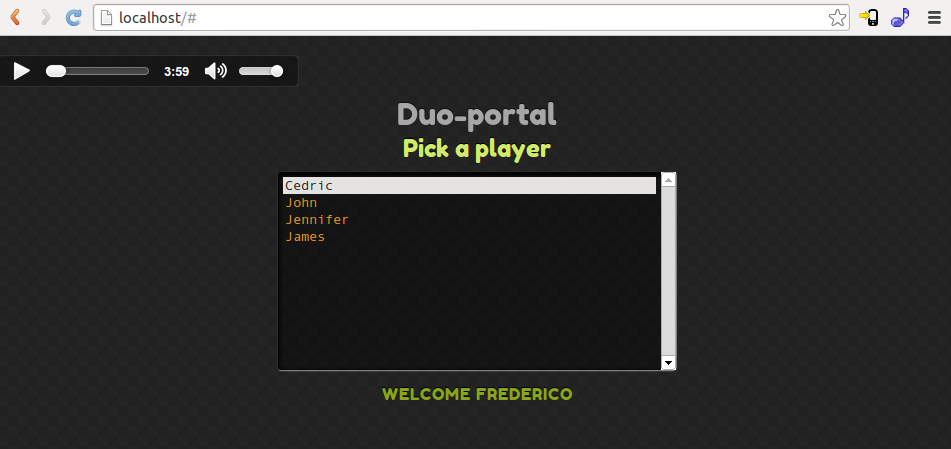
\includegraphics[width=1.4\columnwidth]{index.png}
  \caption{A screenshot of the game}
  \label{fig:index}
}
\end{figure}

\begin{figure}
\hspace*{-0.4\columnwidth}% displace figure
\parbox{1.4\columnwidth}{
  \centering
  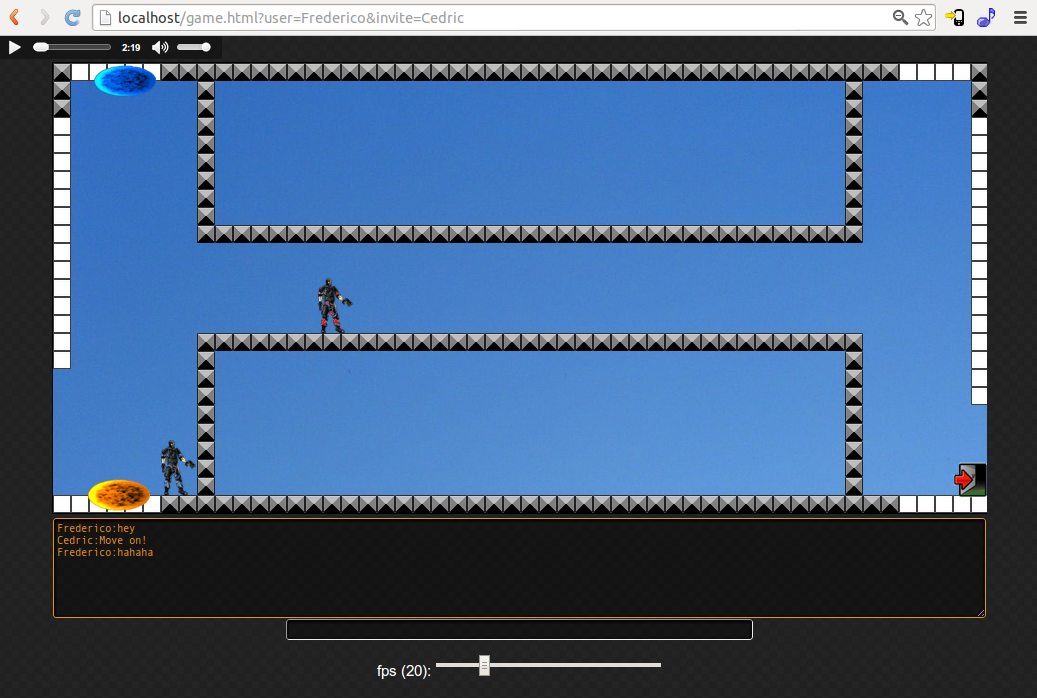
\includegraphics[width=1.4\columnwidth]{game.png}
  \caption{A screenshot of the game}
  \label{fig:game}
}
\end{figure}

\section{Design principles}
We decided to rely on Crafty, a HTML5 game engine in order to code the game. The players first need to connect to the server hosting the game. Then, they are shown a list of players that they can play with. After inviting a player, the game is starting.\\
The players are immersed on the playing platform and have to reach the exit door in order to proceed to the next level. To do so, each of them has a portal and those 2 portals must be combined in order to go further into the level. What stands between the players and the exit door is a set of two kinds of walls. The "white" walls allow players to set their portal on it while the "black" walls do not allow it. This type of wall adds difficulty to the levels by forcing the players to think more carefully where they want to set their portals.\\
We designed the game to be casual. Consequently:\\
\begin{itemize}
\item The gameplay is very simple: you just need to use common commands to move around the game space.
\item The games do not last more than a couple of minutes (and most of the time, they will only last for 30 seconds).
\item Anybody can play these games as they are very simple. The fun of it comes from the communication between players but not from the complexity of the game.
\item You just need to launch a web browser, connect to the web site, invite a friend, and you are playing!
\end{itemize}

\subsection{Manual user}
This manual user can also be found on the login page so that they know what commands to use ingame.
\begin{itemize}
\item Use right and left arrow for walking in a direction.
\item Space for jumping.
\item Right click for opening your portal on "white" walls ("black" walls cannot be targeted).
\end{itemize}

\section{Implementation Details}
The implementation of this paper's work can be divided into three main categories: homepage, network and game mechanics. In this section they are described in details.

\subsection{Homepage}
When accessing the server where the game is hosted, the game's first page is a registration page. To be registered a player just need to give a non-repeated nickname. After entering a nickname the player is welcomed by a message and faces a list with all the players connected to the server but not playing yet. This can be seen in figure \ref{fig:index}.

\subsection{Network implementation}
As this work is a multi-player cooperative casual game it is fundamental to it's working the implementation of a network layer to ensure that one player's action is send to the other player's screen in real time. To achieve this requirement we used websockets \cite{websockets}, a new technology embedded in HTML5 standard. To facilitate the implementation of the network layer we used node.js \cite{nodejs}, a fast and secure javascript platform built using google chrome's javascript runtime API.

Nodejs creates a non-blocking environment for asynchronous requests through the network, this is fundamental for any application that requires a significant number of packets being send through the network per second. In this game the user has the ability to change how many requests per second are performed as shown in the FPS field in figure \ref{fig:game}. After a lot of tests we discovered that 20 requests per second is enough to provide a realistic movement effect of the game and at the same time do not overload the network.

In addition to the ability of change how many requests per second are performed, players can also chat with each other through a simple message field bellow the game section. The chat was implemented in a manner that when players are moving and opening portals they don't need to click in the chat field to communicate, the focus is always in the chat field. In other words, when players want to chat they just need to type the message and press enter. A simple chat between players is demonstrated in figure \ref{fig:game}.

\subsection{Game mechanics implementation}
The Crafty game engine relies on two types of objects: the components and the entities. The components allow to add behaviors to the entities (eg, the DOM component allows the player entity to be displayed on the map).
\newline
\newline
The game is built around a number of components.
\newline
First of all, every object is displayed by using the built-in component DOM, and is given a position with the 2D built-in component. All the collision are handled by the Collision component and its "onHit" method (based on the size of the colliding components).
\newline
The players' motion is specifically handled through the "Ape" component. The main feature of it is to animate the player when it is walking or jumping with the "SpriteAnimation.animate" method.
\newline
The "ParticleCollision" component is used to place a portal on a wall. It uses a particule that will detect collisions on the line formed by the player's arm and the mouse cursor. If a collision happens with an "active" wall (component "active_wall"), the portal will be displayed. Once BOTH portals have been set, the "Teleport" component will take care of transporting the players from one portal to the other. The portals themselves have a vertical or horizontal attribute in order to display them properly on the walls.
\newline
To complete a level, a collision between one of the players and the exit door is enough.
\newline
Finally, graphics are all based on the Sprite component in Crafty that allows to retrieve images associated to objects.
\newline

\section{Design Evolution}
\subsection{During the game coding}
The mechanics of the game took longer than expected (one member of the team had only a limited knowledge of javascript) because the Crafty engine sometimes lacked of references.\\
During the development of the game, we focused on the mechanics rather than the graphics. As neither of us is a game graphic artist, we switched from the mechanics to the graphics near the end of the game development. This means than we had to move from a seamless idea of the graphics to a much more basic way of handle them. Additionaly, we had no IDE nor framework specifically designed to help us with the graphics. For that reason, we reduced the scope of the graphics handling (eg, the player does not move in a natural manner).\\
The network features were implemented in the time that we had planed for. However, interfacing the network features and the game mechanics provided a couple of challenges, coming mainly from the game engine.

\subsection{Designing the levels}
Once the game was operational, we started to work on the level design. We easily came up with 3 levels, but once they were implemented, finding new interesting designs of our own was pretty difficult. We came to understand that coding a game and actually implementing an interesting user experience are two very distinct areas. That is why we decided to stick with 3 levels as a good start for further work on the game.

\section{Discussion and Conclusion}

\balance
\bibliographystyle{acm-sigchi}
\bibliography{sample}

\end{document}
